\documentclass[final,xcolor={dvipsnames,svgnames,x11names,table}]{beamer}
\usetheme{RJH}
%\usetheme{Boadilla}
%\usepackage[orientation=portrait,size=a1,scale=1.3]{beamerposter}
\usepackage[orientation=portrait, size=custom, width=70, height=90, scale=1]{beamerposter}
\usepackage[absolute,overlay]{textpos}
\usepackage{pifont}
\usepackage{ulem}
\usepackage{bm}
\usepackage{siunitx}
\usepackage[export]{adjustbox}
\usepackage{gmp}
\usepackage{smartdiagram}
\usesmartdiagramlibrary{additions}
\usepackage{booktabs}
%\usepackage{enumitem}

%\DeclareGraphicsRule{.1}{mps}{*}{}

\usepackage[listings,theorems]{tcolorbox}


\usepackage{libertine}
\setlength{\TPHorizModule}{1cm}
\setlength{\TPVertModule}{1cm}

\usepackage{tikz,tikz-3dplot} %nalipour
\usetikzlibrary{shapes,arrows, decorations.pathreplacing}%, snakes} %nalipour

\def\Put(#1,#2)#3{\leavevmode\makebox(0,0){\put(#1,#2){#3}}}

% Raised Rule Command:
%  Arg 1 (Optional) - How high to raise the rule
%  Arg 2            - Thickness of the rule
\newcommand{\raisedrule}[2][0em]{\leaders\hbox{\rule[#1]{1pt}{#2}}\hspace{13.5cm}}

\newcommand{\dotrule}[1]{%
   \parbox[]{#1}{\dotfill}}

\setbeamertemplate{bibliography entry title}{}
\setbeamertemplate{bibliography entry location}{}
\setbeamertemplate{bibliography entry note}{}
\footer{}


% \usebackgroundtemplate{%%\includegraphics[width=\paperwidth]{Figures/CLIC_canvas_accelerator_small.jpg}}


\title{\Huge{Design of a drift chamber tracking system for the IDEA experiment at FCC-ee}}
\author{\vspace*{1.5cm}{\Large{Niloufar Alipour Tehrani (CERN), Benedikt Hegner, Giovanni Francesco Tassielli, Francesco Grancagnolo}\\\vspace*{1cm}{\Large{2018 IEEE Nuclear Science Symposium and Medical Imaging Conference}}}}
% \footer{}
\institute{CERN}
\date{}
%\footimage{}

% \usepackage[backend=bibtex,style=numeric-comp,firstinits=true]{biblatex}
% \bibliography{bib}
% \setbeamertemplate{bibliography item}[text]
% \renewcommand*{\bibfont}{\footnotesize}

% tcolorbox styles
\tcbset{%
    noparskip,
    colback=white, %background color of the box
    colframe=i6colorblockbg, %color of frame and title background
    coltext=black, %color of body text
    coltitle=white, %color of title text
    fonttitle=\bfseries,
    alerted/.style={coltitle=red,
                     colframe=gray!40},
    subtcolorbox/.style={coltitle=black,
                     colframe=i6colorscheme3,
                     colback=white,
                     coltitle=i6colorblockbg},
    }


\begin{document}
\begin{frame}

\begin{textblock}{2}(0.8,0.25)

\includegraphics[width=4.\textwidth]{Figures/logo_cern.pdf}
\end{textblock}
\begin{textblock}{6}(61,0.01)

\includegraphics[width=1.5\textwidth]{Figures/FCC-logo}
\end{textblock}
\begin{textblock}{20}(4.5, 11)
%\textcolor{red}{\small{\url{http://clicdp.web.cern.ch/}}}
\end{textblock}


%%%%%%%%%%%%%%%%%%%%%%%%%%%%%%%%%%%%%
%%%                             Block                                %%%
%%%%%%%%%%%%%%%%%%%%%%%%%%%%%%%%%%%%%
\begin{textblock}{16.5}(0.5, 14)
  \begin{tcolorbox}[title=FCC: Future Circular Collider]

  \begin{itemize}
    \item A future collider
    \item 3 options
  \end{itemize}
    \centering
    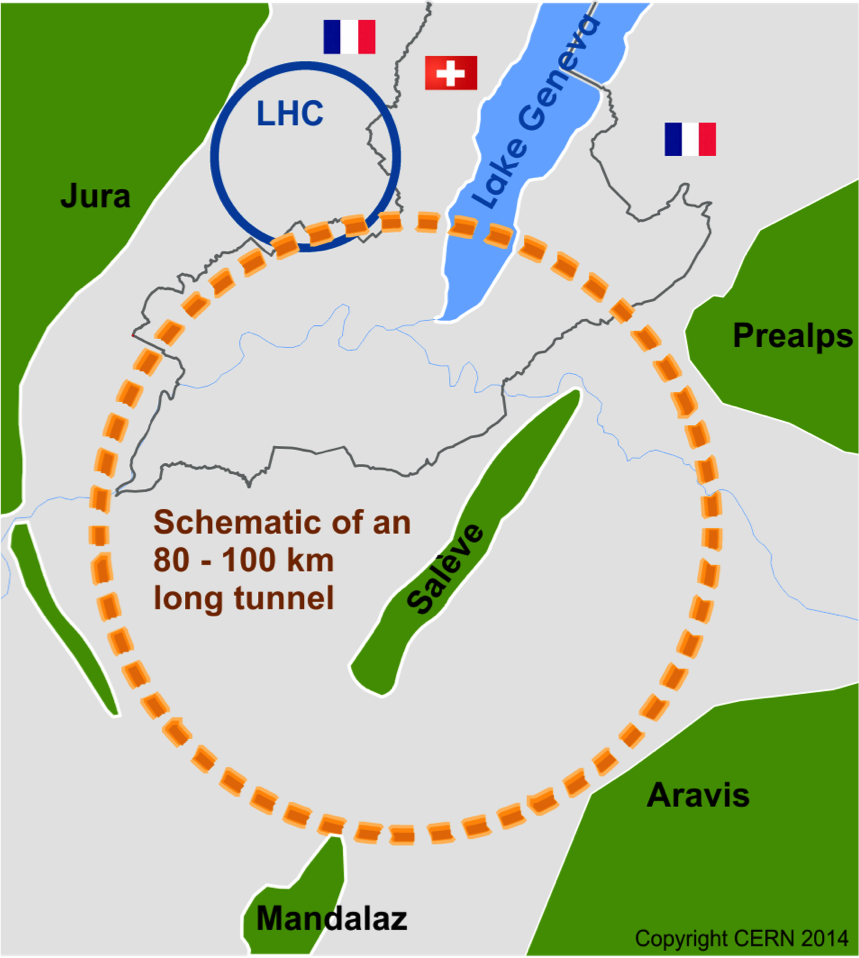
\includegraphics[width=0.9\textwidth]{Figures/cernFCC}

  \end{tcolorbox}
\end{textblock}
%
% %%%%%%%%%%%%%%%%%%%%%%%%%%%%%%%%%%%%%
% %%%                             Block                 %%%
% %%%%%%%%%%%%%%%%%%%%%%%%%%%%%%%%%%%%%
\begin{textblock}{52}(17.5, 14)
  \begin{tcolorbox}[title=FCCSW: Physics and Detector simulations with FCCSW]

  \centering
  	\smartdiagramset{back arrow disabled=true}
  	% \scalebox{5}{
  	  	\smartdiagram[flow diagram:horizontal]
  	  	{%
  	    	{Geometry\\DDhep}, Segmentation, {Geant4 \\simulation}, Digitization%
  	  	}
    	% }

  \end{tcolorbox}
\end{textblock}
% %%%%%%%%%%%%%%%%%%%%%%%%%%%%%%%%%%%%%
% %%%                             Block                                %%%
% %%%%%%%%%%%%%%%%%%%%%%%%%%%%%%%%%%%%%
\begin{textblock}{36.8}(22, 27)
  \begin{tcolorbox}[title=The IDEA detector concept]

  \centering
  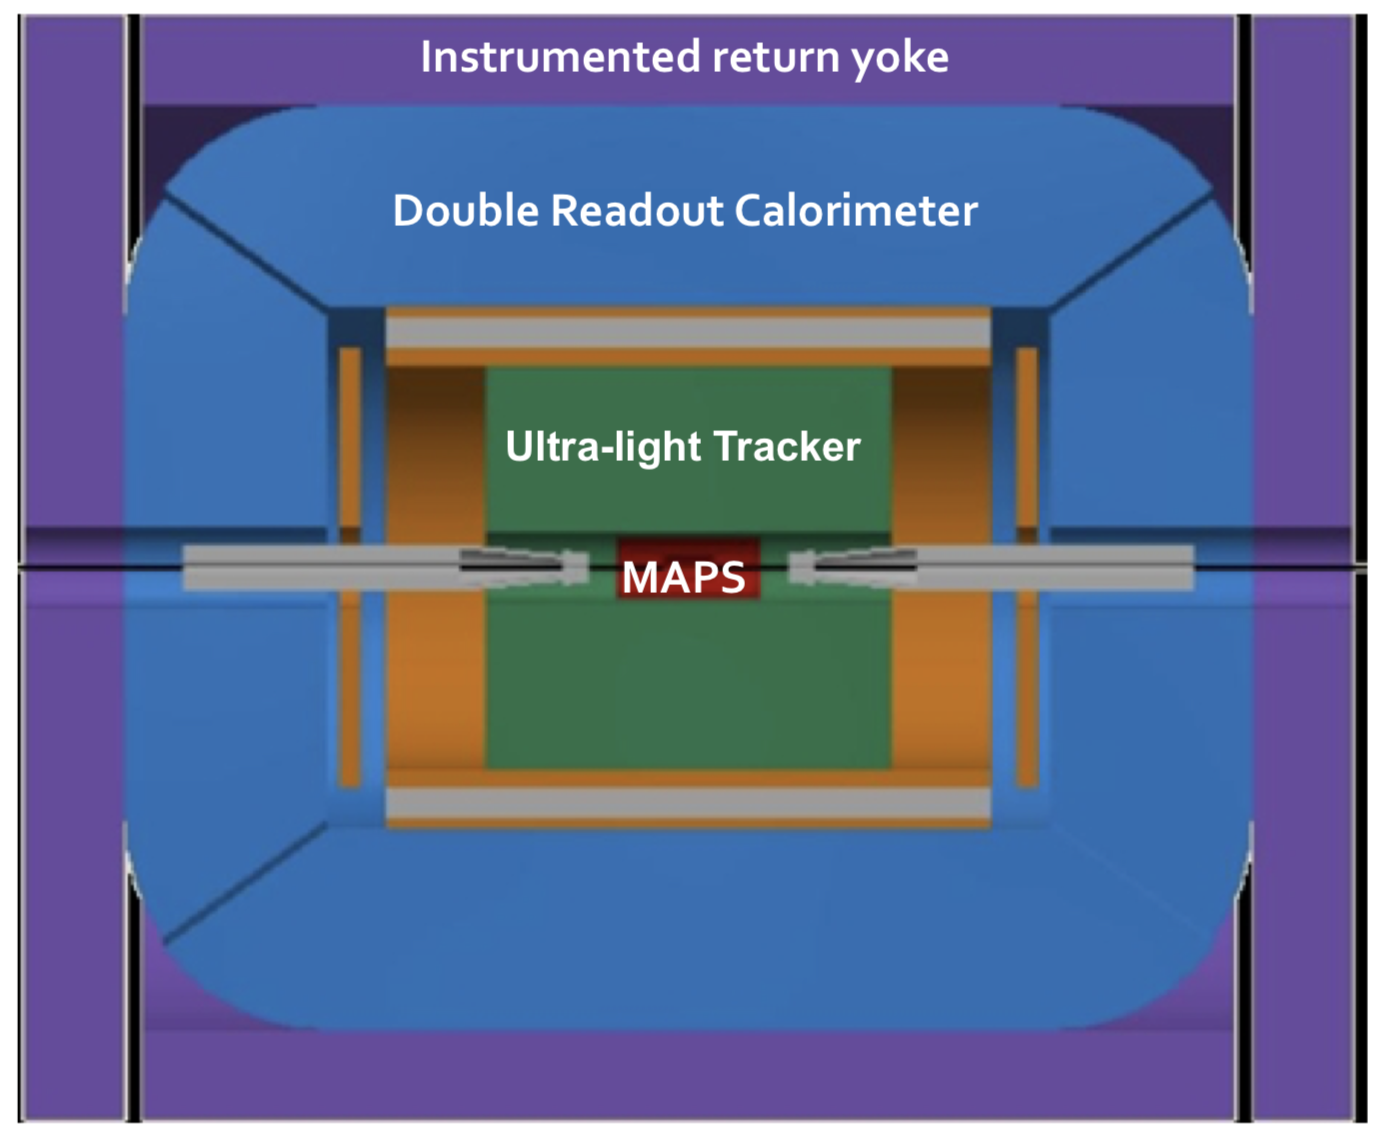
\includegraphics[width=0.5\textwidth]{../figures/FCCeeIDEAConcept}

  \end{tcolorbox}
\end{textblock}

%%%%%%%%%%%%%%%%%%%%%%%%%%%%%%%%%%%%%
%%%                             Block                                %%%
%%%%%%%%%%%%%%%%%%%%%%%%%%%%%%%%%%%%%
\begin{textblock}{69}(0.5, 36.5)
  \begin{tcolorbox}[title=Simulation of the drift chamber within FCCSW]

  \begin{columns}
  \column{0.33\textwidth}
    \begin{tikzpicture}
      \node[anchor=south west,inner sep=0] (image) at
      (0,0){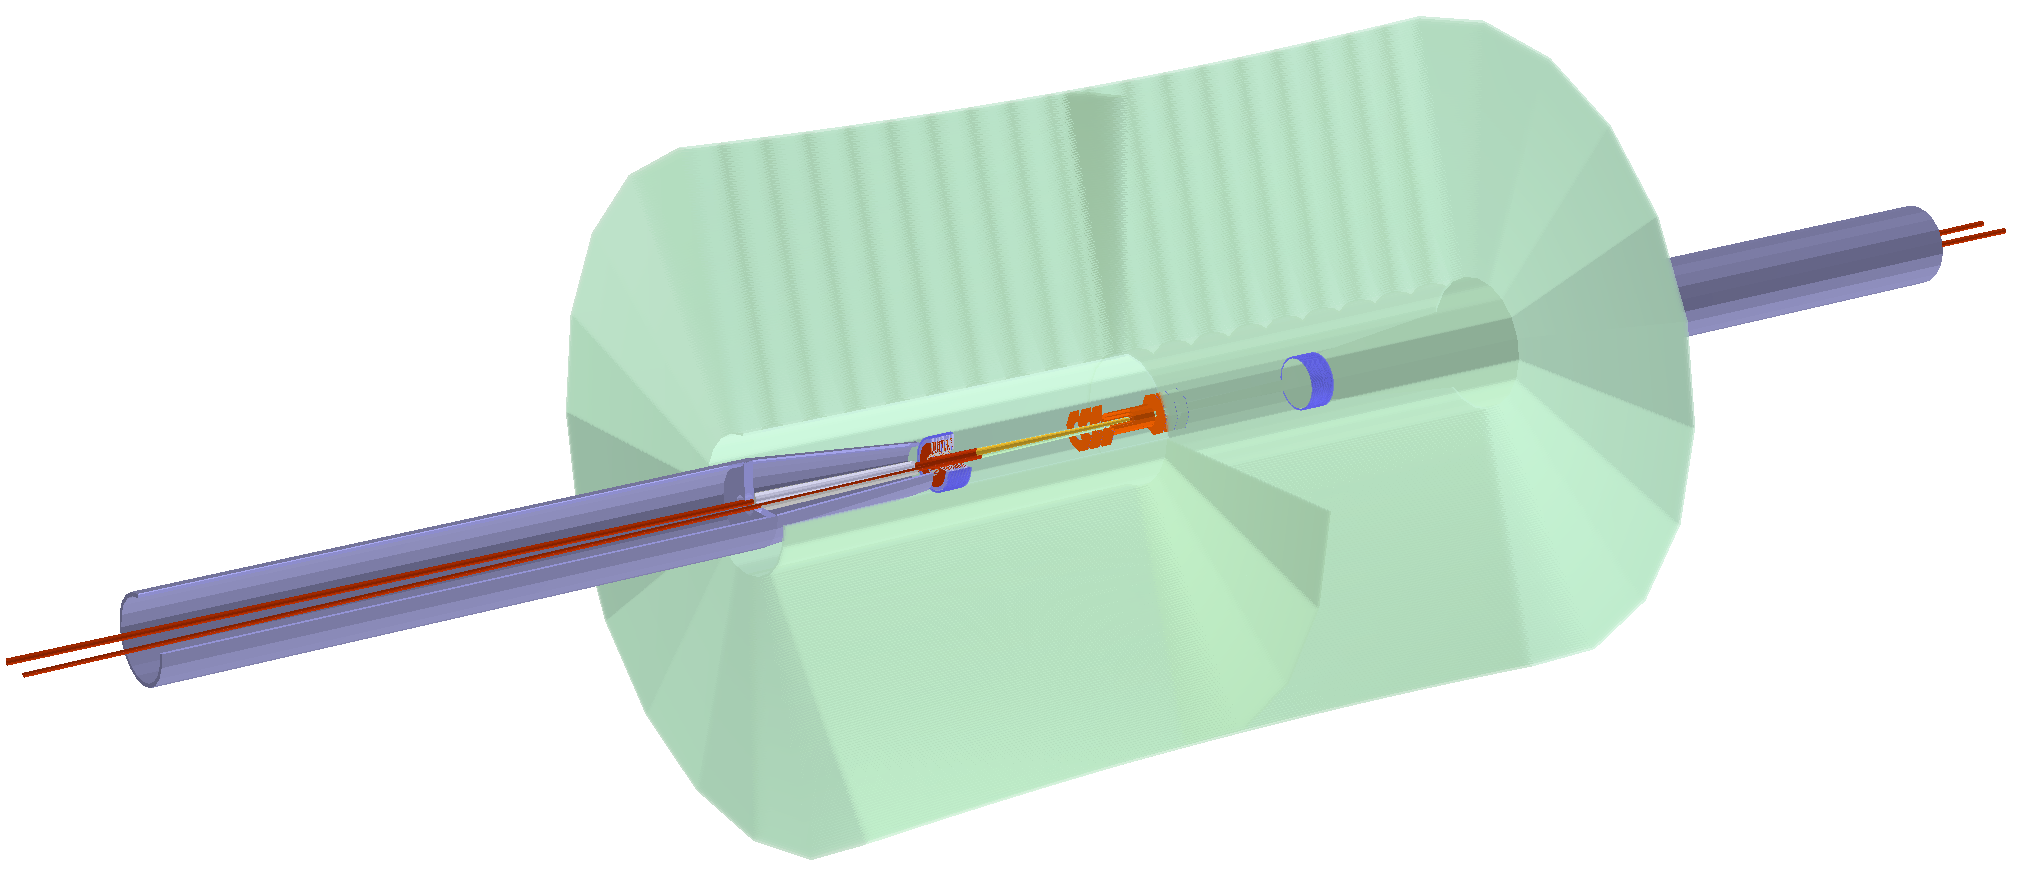
\includegraphics[width=5in]{../figures/FCCeeIDEA_IR}};
      \begin{scope}[x={(image.south east)},y={(image.north west)}]

      \draw[->, thick](0.2, 0.7) -- (0.4, 0.7);
      \node[left] at (0.2, 0.7) {Drift chamber};

      \draw[->, thick](-0.1, 0.25) -- (0., 0.25);
      \node[left] at (-0.1, 0.25) {Beam pipe};

      \draw[->, thick](0.1, 0.4) -- (0.2, 0.4);
      \node[left] at (0.1, 0.4) {Solenoid shielding};

      \draw[->, thick](0.6, 0.05) -- (0.48, 0.4);
      \node[below] at (0.6, 0.05) {Luminosity calorimeter};

      \draw[->, thick](0.8, 0.2) -- (0.58, 0.5);
      \node[below] at (0.8, 0.2) {Vertex detector};

      \end{scope}
    \end{tikzpicture}

  \column{0.33\textwidth}
    \centering
    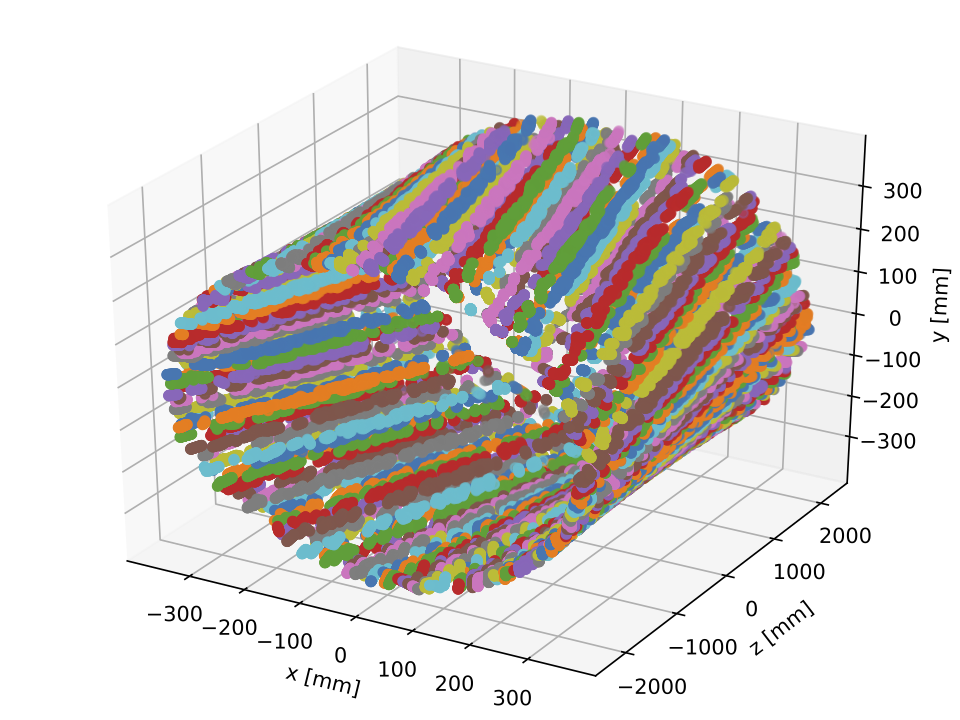
\includegraphics[width=5in]{Figures/allHits}

  \column{0.33\textwidth}
    \centering
    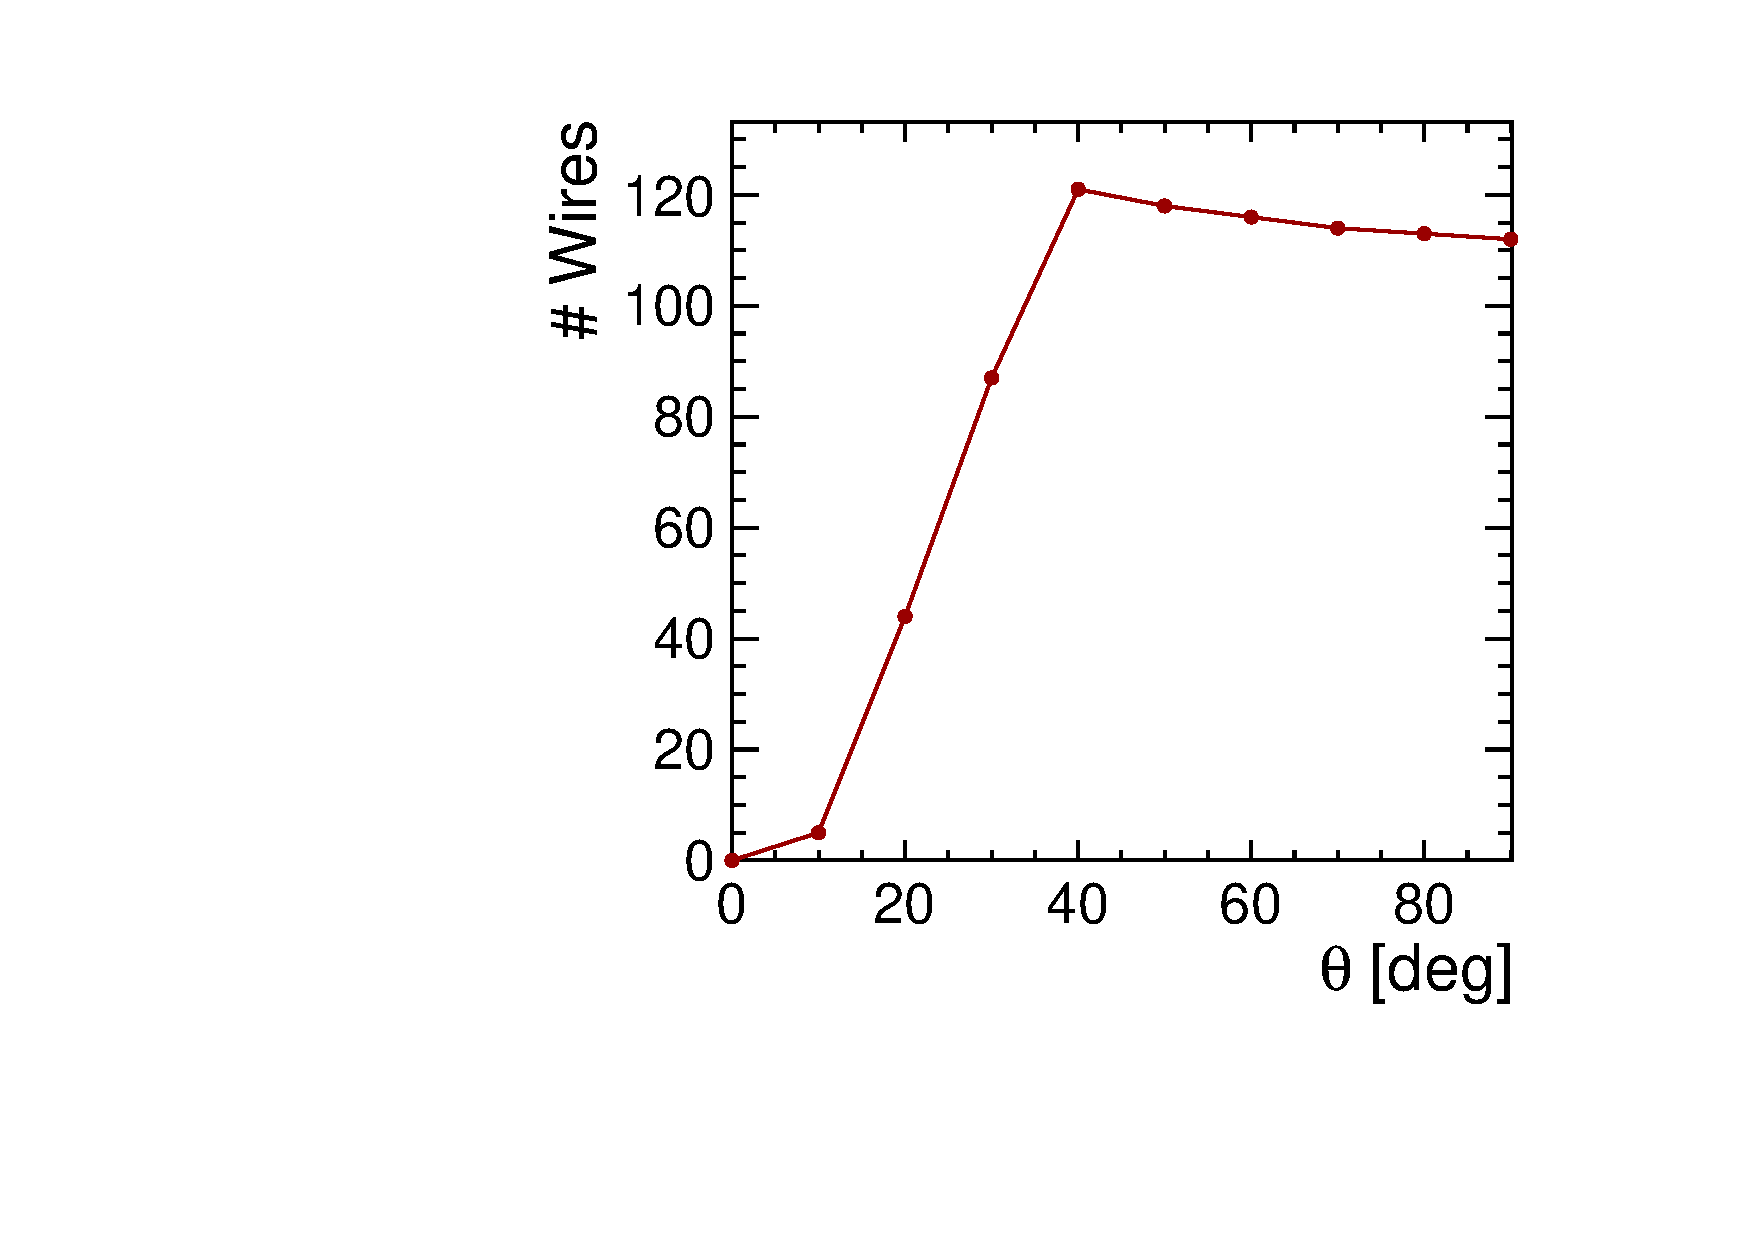
\includegraphics[width=5in]{Figures/numWires}

  \end{columns}


  \end{tcolorbox}
\end{textblock}

%%%%%%%%%%%%%%%%%%%%%%%%%%%%%%%%%%%%%
%%% Block %%%
%%%%%%%%%%%%%%%%%%%%%%%%%%%%%%%%%%%%%
\begin{textblock}{34.2}(0.5, 50)
  \begin{tcolorbox}[title=Beam-induced backgrounds]

  \begin{columns}
    \column{0.5\textwidth}

    \column{0.5\textwidth}
    \centering
    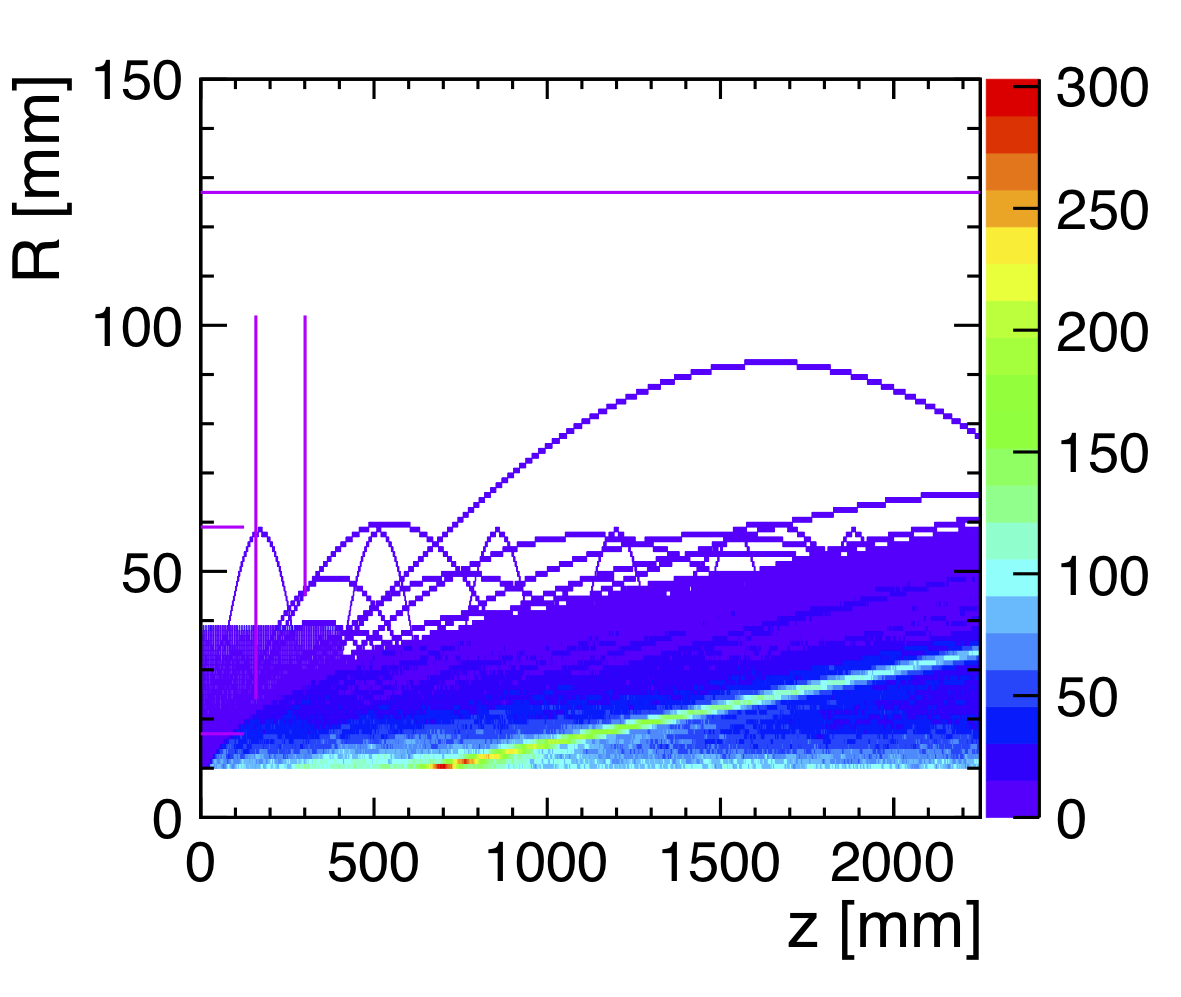
\includegraphics[width=5in]{../figures/pairs_R_Z}
  \end{columns}

  \end{tcolorbox}
\end{textblock}

%%%%%%%%%%%%%%%%%%%%%%%%%%%%%%%%%%%%%
%%% Block %%%
%%%%%%%%%%%%%%%%%%%%%%%%%%%%%%%%%%%%%
\begin{textblock}{34.2}(35, 50)
  \begin{tcolorbox}[title=Beam-induced backgrounds]

  \centering
	\begin{tabular}{l c c}
  	\toprule
	   Background & \multicolumn{2}{c}{Average occupancy} \\
	    & E\textsubscript{cm} = 91.2~GeV &  E\textsubscript{cm} = 365~GeV \\
	   \midrule
	   $e^+e^-$ pair background & 1.1\% & 2.9\% \\
	   $\gamma\gamma\rightarrow$ hadrons & 0.001\% & 0.035\%  \\
	   Synchrotron radiation & - & 0.2\% \\
	   \bottomrule
	\end{tabular}

  \end{tcolorbox}
\end{textblock}

%--------------------------------------------%
\end{frame}
\end{document}
